\documentclass[12pt]{article}
\usepackage{amsmath}
\usepackage{gensymb}
\usepackage{float}
\usepackage{graphics}
\usepackage{graphicx}
\graphicspath{storage/self/primary/Download/assignment/fig}
\let\vec\mathbf
\providecommand{\abs}[1]{\ensuremath{\left|#1\right|}}
\providecommand{\norm}[1]{\ensuremath{\lVert#1\rVert}}
\providecommand{\brak}[1]{\ensuremath{\left(#1\right)}}
\begin{document}
\title{\textbf{ASSIGNMENT 2}}
\date{}
\maketitle
\textbf{Question :} Two lines passing through the point(2,3) intersect each other at an angle of $60\degree$.If slope of one line is 2,find equation of the other line.

\textbf{Solution :} The equation of one line having slope 2 is
\begin{align}
    \brak{y-3}=2\brak{x-2}\\
    or,2x-y=1
\end{align}
So,the normal vector is,$\vec{n_1}=\begin{pmatrix}
    2\\-1
\end{pmatrix}$

Let the slope of another line is $m$.
So,the equation of the line is
\begin{align}
    \brak{y-3}=m\brak{x-2}\\
    or,mx-y=2m-3
\end{align}
So, the normal vector is,$\vec{n_2}=\begin{pmatrix}
    m\\-1
\end{pmatrix}$
\begin{align}
	\cos{60\degree}&=\frac{\vec{n_1n_2}}{\vec{\norm{n_1}\norm{n_2}}}\\
    \frac{1}{2}&=\frac{\begin{pmatrix}
        2\\-1
    \end{pmatrix}\begin{pmatrix}
        m\\-1
    \end{pmatrix}}{\sqrt{5}\sqrt{m^2+1}}\\
    \frac{1}{2}&=\frac{2m+1}{\sqrt{5m^2+5}}\\
    m&=\frac{-8\pm5\sqrt{3}}{11}
\end{align}
So,the equation of the line is
\begin{align}
    \brak{y-3}&=\frac{-8-5\sqrt{3}}{11}\brak{x-2}\\
    \brak{y-3}&=\frac{-8+5\sqrt{3}}{11}\brak{x-2}\\
\end{align}


\textbf{Figure :}
\begin{figure}[H]
    \centering
    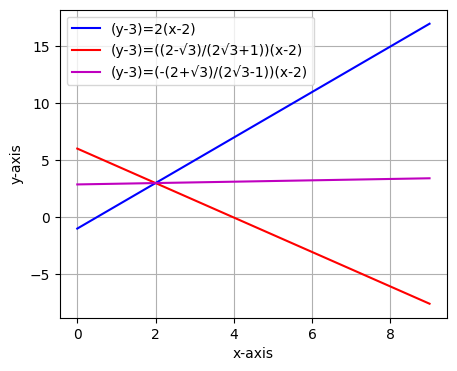
\includegraphics[width=\columnwidth]{fig/asgnt.png}
    \caption{Required Figure}
    \label{fig:fig:1}
\end{figure}
\end{document}

